\chapter{Analisis}
\label{chap:analysis}
\vspace{-1em} % prevent widow on second next pages
\section{Analisis Aplikasi Sejenis}
\label{sec:analysis-similarapps}

Untuk pembuatan perangkat lunak dalam skripsi ini, ada empat buah perkakas \cl\xspace yang akan diamati sebagai aplikasi sejenis. Dua dari empat aplikasi pertama adalah \chromewebstorecli\xspace dan \itunesapi. Selain dua perkakas tersebut, ada dua perkakas lainnya yang bisa digunakan sebagai referensi, tetapi tidak dapat dieksplorasi, karena kedua aplikasi tersebut tidak berhasil dijalankan dengan sempurna, yaitu \ubercli\xspace dan \googlemapscli. Keempat perkakas ini akan dilihat dan diteliti untuk analisis bagaimana format serta karakteristik opsi-opsi dari perkakas \cl\xspace pada umumnya.
\vspace{-0.15em} % prevent widow on second next pages
\subsection[\chromewebstorecli]{\chromewebstorecli\footnote{\href{https://github.com/pandawing/node-chrome-web-store-item-property-cli}{https://github.com/pandawing/node-chrome-web-store-item-property-cli}, versi 2.0.1}}
\label{sec:similarapps-chromewebstore}

Perkakas pertama yang akan diteliti adalah \chromewebstorecli\xspace yang dibuat oleh pengguna GitHub dengan nama ``pandawing''. Perkakas ini merupakan ekstensi dari sebuah aplikasi lain (dari pembuat yang sama) yang memiliki fungsi yang sama, yaitu Chrome \textit{Web Store Item Property}\footnote{\href{https://github.com/pandawing/node-chrome-web-store-item-property}{https://github.com/pandawing/node-chrome-web-store-item-property}, versi 1.2.0}. Artinya, perkakas ini memiliki fungsi yang sama dengan aplikasi dasarnya, yaitu memanggil fungsi API untuk mendapatkan metadata dari sebuah ekstensi pada \textit{web store} peramban Google Chrome. Perbedaan dari perkakas ini dengan aplikasi dasarnya adalah bahwa perkakas ini dapat digunakan sebagai perkakas \textit{command line}, sedangkan aplikasi dasarnya hanya bisa digunakan dalam perangkat lunak lainnya sebagai pemanggil fungsi API.
\vspace{-0.15em} % prevent widow on second next pages
\subsubsection{Penggunaan}
\label{sec:similarapps-chromewebstore-usage}

Perkakas ini dapat digunakan melalui \textit{command prompt} dengan cara mengetikkan perintah sebagai berikut.

\begin{verbatim}
                   chrome-web-store-item-property <identifier>
\end{verbatim}

Dengan \verb|identifier| berupa ID dari ekstensi yang diinginkan. Jadi, misalkan pengguna memasukkan \verb|gighmmpiobklfepjocnamgkkbiglidom| sebagai ID yang akan digunakan sebagai \textit{identifier}, maka perkakas ini akan mengembalikan metadata dari ekstensi ``AdBlock'' sebagai keluarannya. Contoh penggunaan perkakas ini dapat dilihat di Gambar \ref{fig:similarapps-chromewebstorecli-usage}.

\begin{figure}[ht]
    \centering
    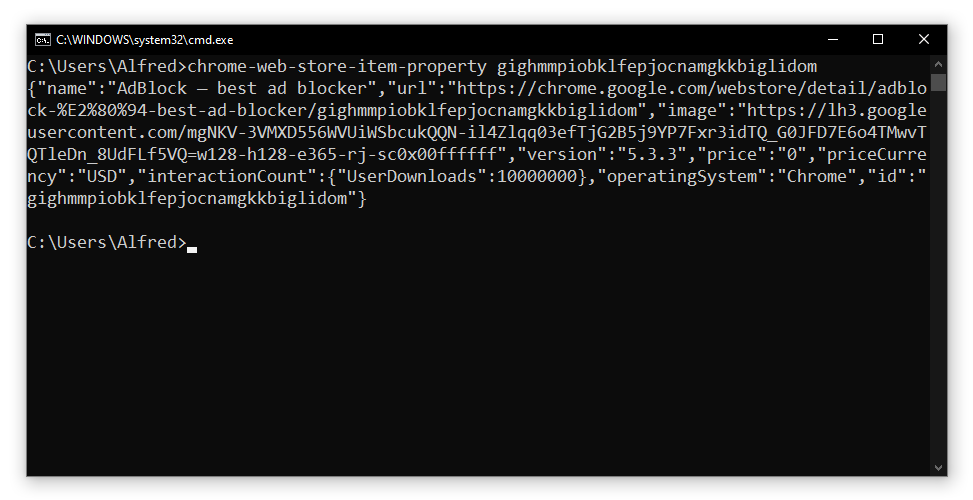
\includegraphics[width=0.95\linewidth]{chromewebstorecli-usage}
    \caption[Contoh penggunaan perkakas \chromewebstorecli]{Contoh penggunaan perkakas \chromewebstorecli\xspace untuk mencari ekstensi ``AdBlock''.}
    \label{fig:similarapps-chromewebstorecli-usage}
\end{figure}

Sedangkan, keluaran dari perkakas ini merupakan sebuah objek JSON dengan properti-properti sebagai berikut.

\begin{itemize}
	\item \verb|name|\\
	Nama dari ekstensi yang dicari \textit{metadata}-nya.
	\item \verb|url|\\
	URL halaman web dari ekstensi yang dicari di \textit{web store} Google Chrome.
	\item \verb|image|\\
	Logo (dan ikon \textit{thumbnail}) dari ekstensi yang dicari \textit{metadata}-nya.
	\item \verb|version|\\
	Nomor versi dari ekstensi.
	\item \verb|price|\\
	Harga dari ekstensi. Jika ekstensi tidak memiliki harga yang perlu dibayarkan (gratis), properti ini akan bernilai \verb|0|.
	\item \verb|priceCurrency|\\
	Kode mata uang dari harga ekstensi. Jika ekstensi tidak memiliki harga yang perlu dibayarkan, properti ini akan berisi ``\verb|USD|''.
	\item \verb|interactionCount|\\
	Properti ini berisi interaksi-interaksi pengguna yang tercatat sebagai data di halaman \textit{web store} ekstensi. Pada saat pembuatan skripsi ini, properti ini hanya memiliki satu buah subproperti, yaitu \verb|userDownloads|, yang menandakan berapa kali ekstensi ini telah diunduh oleh pengguna di mana pun.
	\item \verb|operatingSystems|\\
	Menandakan di peramban mana ekstensi versi ini dapat diinstal. Karena ekstensi-ekstensinya berada di \textit{web store} Chrome,
	\item \verb|ratingValue| (tidak digunakan lagi)\\
	Peringkat yang diberikan oleh para pengguna ekstensi ini. Nilai dari properti ini berupa skala desimal dari 0.00 sampai dengan 5.00. Di versi terbaru dari perkakas ini, properti ini tidak lagi tersedia dalam keluarannya.
	\item \verb|ratingCount| (tidak digunakan lagi)\\
	Jumlah pengguna yang telah menilai/memberi peringkat ke ekstensi ini. Di versi terbaru dari perkakas ini, properti ini tidak lagi tersedia dalam keluarannya.
	\item \verb|id|\\
	Properti ini mengandung ID dari ekstensi tersebut. Nilai dari properti ini akan sama dengan ID yang digunakan sebagai parameter masukan perkakas.
\end{itemize}
\noindent
Selain penggunaan normalnya, pengguna perkakas ini juga dapat meminta perkakas untuk menampilkan halaman bantuannya, yaitu dengan perintah sebagai berikut.
\vspace{-0.025em} % prevent widow
\begin{verbatim}
                     chrome-web-store-item-property --help
\end{verbatim}
\vspace{-0.025em} % prevent widow
\noindent
Hasil dari eksekusi perintah ini dapat dilihat di Gambar \ref{fig:similarapps-chromewebstorecli-help}.

\begin{figure}[ht]
    \centering
    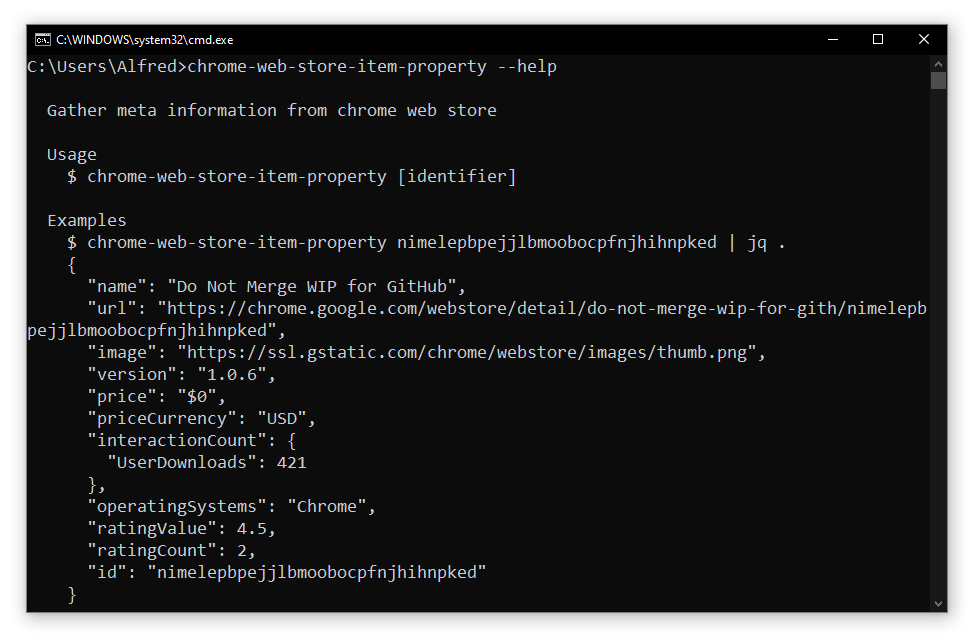
\includegraphics[width=0.95\linewidth]{chromewebstorecli-help}
    \caption[Opsi bantuan penggunaan pada perkakas \chromewebstorecli]{Opsi \texttt{-{}-help} pada perkakas \chromewebstorecli.}
    \label{fig:similarapps-chromewebstorecli-help}
\end{figure}

\subsection[\itunesapi]{\itunesapi\footnote{\href{https://github.com/awcross/itunes-search-api}{https://github.com/awcross/itunes-search-api}, versi 1.0.1}}
\label{sec:similarapps-itunesapi}

Perkakas kedua yang akan diteliti adalah \itunesapi\xspace oleh pengguna GitHub dengan nama ``awcross''. Perkakas ini berfungsi untuk melakukan pencarian dengan mengutilisasikan API iTunes, sehingga seakan-akan pengguna langsung melakukan pencarian di iTunes sendiri. Hasil pencarian yang dilakukan termasuk judul lagu, nama artis, ataupun nama album, dan pengguna dapat memilih secara spesifik objek apa yang ingin dicari.

\subsubsection{Penggunaan}
\label{sec:similarapps-itunesapi-usage}

Perkakas ini dapat digunakan melalui \textit{command prompt} dengan cara mengetikkan perintah sebagai berikut.

\begin{verbatim}
                      itunes-search-api <input> [<options>]
\end{verbatim}

Dengan \verb|input| berupa nama dari objek yang dicari. Perkakas ini juga memiliki opsi yang masing-masing memiliki parameter tersendiri untuk mempersempit hasil pencarian. Adapun opsi-opsi tersebut dapat dilihat di daftar di bawah ini.

\begin{figure}[h]
    \centering
    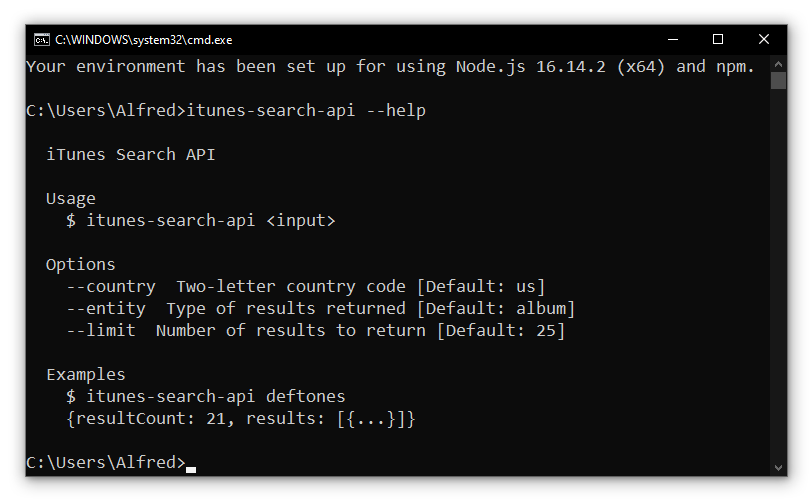
\includegraphics[width=0.8\linewidth]{itunesapi-help}
    \caption[Opsi bantuan penggunaan pada perkakas \itunesapi]{Opsi \texttt{-{}-help} pada perkakas \itunesapi.}
    \label{fig:similarapps-itunesapi-help}
\end{figure}

\begin{itemize}
	\item \verb|--help|\\
	Opsi ini merupakan opsi untuk menampilkan bantuuan penggunaan perkakas, di mana ketika pengguna menjalankan perkakas dengan opsi ini, maka perkakas akan mengeluarkan format penggunaan perkakas, seluruh daftar opsi yang dapat digunakan, serta satu contoh penggunaannya. Adapun penggunaan serta keluaran dari opsi ini dapat dilihat di Gambar \ref{fig:similarapps-itunesapi-help}. Opsi ini juga tidak memiliki argumen apapun yang  (\verb|<options>| tidak perlu diikutkan).
	\item \verb|--country|\\
	\textbf{Kemungkinan nilai:} Kode negara dua huruf\\
	Opsi ini menerima parameter berupa kode negara asal dari album atau artis yang dicari.
	\newpage\vspace*{-1.75em} % fix space at the end of page
	\item \verb|--entity|\\
	\textbf{Kemungkinan nilai:} \verb|song|, \verb|musicArtist|, atau \verb|album|\\
	Menandakan jenis entitas (objek) yang ingin dicari. Opsi ini dapat bernilai \verb|song| untuk pencarian berbasis judul lagu, \verb|musicArtist| untuk pencarian nama artis, atau \verb|album| untuk pencarian nama album. Jika opsi ini tidak dipakai, objek apa pun yang memiliki kemiripan dengan \verb|input| dalam salah satu dari ketiga properti ini akan muncul dalam hasil pencarian.
	\item \verb|--limit|\\
	\textbf{Kemungkinan nilai:} Bilangan bulat positif\footnote{Opsi ini juga menerima bilangan bulat negatif, tetapi menggunakan sebuah bilangan bulat negatif akan menghilangkan pengaruh opsi ini terhadap hasil keluaran.}\\
	Batas maksimal hasil pencarian yang ingin ditampilkan dalam keluaran.
\end{itemize}
\vspace{0.75\baselineskip} % fix space at the end of page
\noindent
Sedangkan, keluaran dari perkakas ini merupakan sebuah objek JSON yang memiliki dua properti utama, yaitu:

\begin{itemize}
	\item \verb|resultCount|\\
	Properti ini berisi bilangan bulat yang menandakan berapa buah objek yang terdapat dalam hasil pencarian.
	\item \verb|results|\\
	\textit{Array} yang berisi kumpulan objek yang terdapat di dalam hasil pencarian. Objek-objek ini akan dikembalikan berupa sebuah \textit{array} lain yang berisi seluruh properti dari masing-masing objek. Apa saja properti yang diikutkan dalam \textit{array} tersebut tergantung tipe dari objek dalam hasil pencarian.
\end{itemize}
\vspace{0.75\baselineskip} % fix space at the end of page
\noindent
Adapun contoh penggunaan dan hasil keluaran perkakas ini dapat dilihat di Gambar \ref{fig:similarapps-itunesapi-usage}.

\begin{figure}[ht]
    \centering
    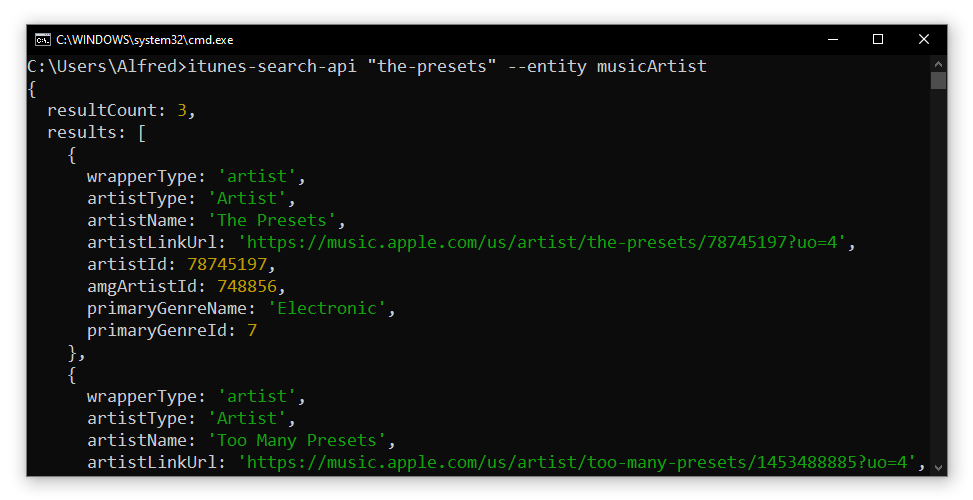
\includegraphics[width=0.95\linewidth]{itunesapi-usage}
    \caption[Contoh penggunaan perkakas \itunesapi]{Contoh penggunaan perkakas \itunesapi\xspace untuk mencari artis bernama ``\textit{The Presets}''.}
    \label{fig:similarapps-itunesapi-usage}
\end{figure}

\subsection[\ubercli]{\ubercli\footnote{\href{https://github.com/jaebradley/uber-cli}{https://github.com/jaebradley/uber-cli}, versi 1.0.2}}
\label{sec:similarapps-ubercli}

\ubercli\xspace merupakan sebuah perkakas \cl\xspace yang dibuat oleh pengguna GitHub dengan nama ``jaebradley''. Perkakas ini yang dapat digunakan untuk dua fungsi utama. Fungsi pertama dari perkakas ini adalah untuk mendapatkan estimasi untuk seberapa lama waktu yang diperlukan untuk servis taksi \textit{online} dari Uber untuk mencapai lokasi yang ingin dituju, sedangkan fungsi \mbox{keduanya} adalah untuk mengestimasi harga yang harus dibayarkan untuk memakai servis tersebut. 
\newpage
\noindent
Fungsi yang pertama dapat dilakukan memanggil perintah dengan format sebagai berikut.

\begin{verbatim}
                                uber time <alamat>
\end{verbatim}

\verb|uber| merupakan perintah dasar dari perkakas ini. \verb|time| merupakan parameter yang menandakan bahwa pengguna ingin menggunakan servis prediksi waktu dari perkakas ini. Selain itu, pengguna harus memasukkan alamat yang ingin dituju sebagai parameter akhir dari perintah yang akan digunakan sebagai masukan. Jika sintaksnya sudah benar, perintah tersebut akan bisa diproses oleh perkakas dengan cara mengirimkan pesan hasil konversi perintah tersebut ke API Uber. Setelah pemrosesan pesan tersebut berhasil, perkakas ini akan menampilkan sebuah keluaran dengan format yang dapat dilihat di Gambar \ref{fig:similarapps-ubercli-time}. Keluaran yang dihasilkan oleh perkakas ini akan meliputi seluruh jenis servis yang disediakan oleh Uber, dan menunjukkan estimasi waktu tempuh perjalanan untuk tiap-tiap servisnya.
\vspace*{1em} % maximize vertical space
\begin{figure}[h]
    \centering
    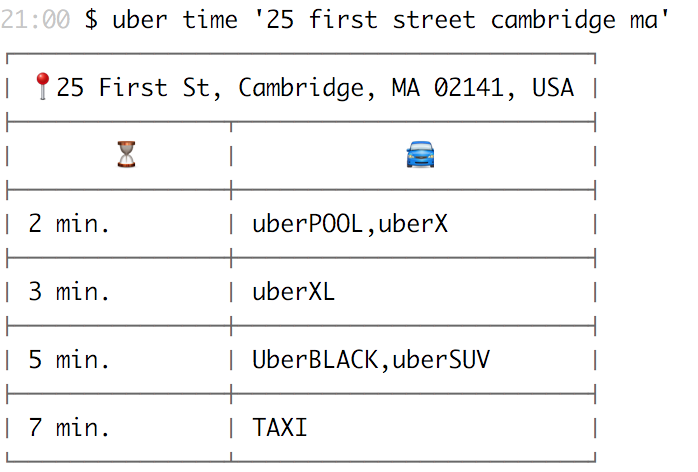
\includegraphics[width=0.5\linewidth]{ubercli-time}
    \caption[Contoh penggunaan perkakas \ubercli (\textit{time})]{Contoh penggunaan fitur prediksi waktu perjalanan untuk perkakas \ubercli.\protect\footnotemark}
    \label{fig:similarapps-ubercli-time}
\end{figure}
\footnotetext{\href{https://github.com/jaebradley/uber-cli}{https://github.com/jaebradley/uber-cli}}
\newpage % maximize vertical space
Hal lain yang perlu diperhatikan bahwa di keluaran perkakas ini ada beberapa gambar grafis. Gambar-gambar ini disebut \textit{emoji unicode}, yang merupakan karakter-karakter \textit{unicode} berupa simbol piktorial (piktograf). Karena pada dasarnya \textit{emoji-emoji unicode} ini merupakan karakter \textit{unicode}, mereka didukung oleh CLI apapun yang mendukung karakter \textit{unicode}\footnote{\href{https://www.unicode.org/emoji/techindex.html}{https://www.unicode.org/emoji/techindex.html}}.

Untuk memanggil fungsi kedua dari perkakas ini, pengguna dapat dilakukan dengan memanggil perintah dengan format berikut.
\vspace{0.25em} % Prevent awkwardly-cut orphans
\begin{verbatim}
                  uber price -s <alamat awal> -e <alamat akhir>
\end{verbatim}
\vspace{0.25em} % Prevent awkwardly-cut orphans
Untuk sintaks ini, \verb|uber| memiliki fungsi yang sama dengan sintaks untuk fungsi pertama dari perkakas. \verb|price| merupakan penanda untuk perkakas bahwa pengguna ingin menggunakan servis untuk mengetahui perkiraan harga layanan Uber. Selanjutnya, perkakas akan meminta dua buah opsi beserta parameternya masing-masing. Pertama, opsi \verb|-s|, berarti \textit{start}, yang akan meminta sebuah parameter berupa lokasi yang ingin dipakai sebagai lokasi awal perkiraan harga layanan Uber. Sedangkan opsi \verb|-e|, berarti \textit{end}, akan meminta sebuah parameter berupa lokasi yang ingin dipakai sebagai lokasi akhir jasa perkiraan harga.

Keluaran dari fungsi kedua ini dapat dilihat di Ggambar \ref{fig:similarapps-ubercli-price}. Sama seperti keluaran untuk fungsi pertamanya, keluaran untuk fungsi kedua perkakas ini juga meliputi seluruh jasa yang disediakan oleh Uber.
\vspace*{1em} % Prevent awkwardly-cut orphans
\begin{figure}[ht]
    \centering
    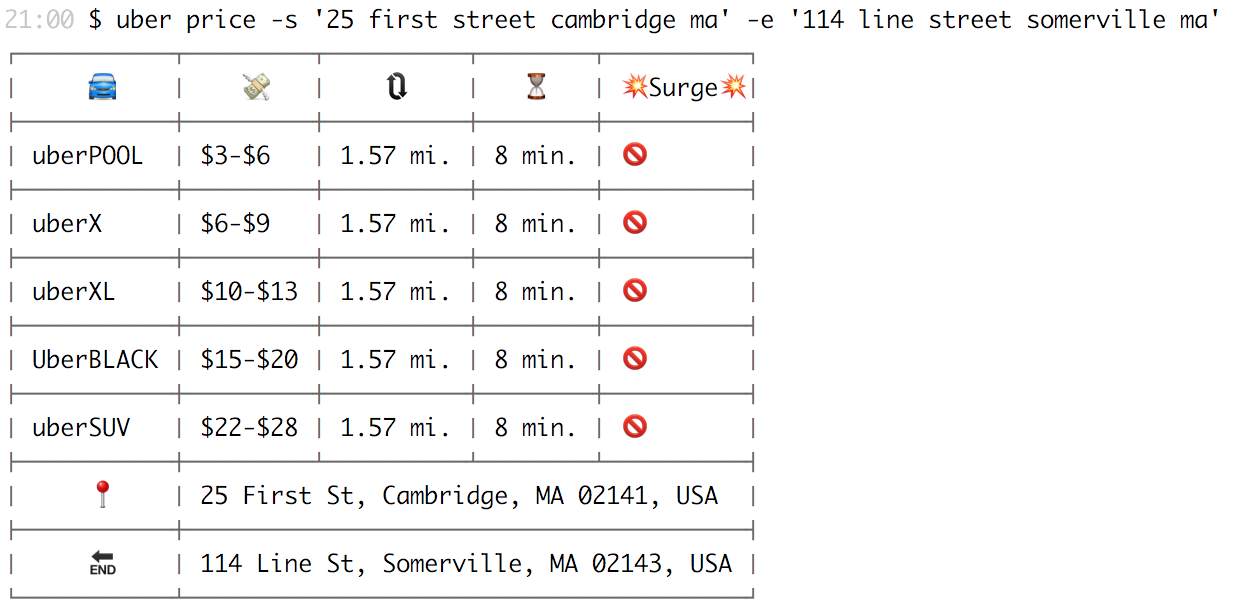
\includegraphics[width=0.9\linewidth]{ubercli-price}
    \caption[Contoh penggunaan perkakas \ubercli (\textit{price})]{Contoh penggunaan fitur prediksi harga perjalanan untuk perkakas \ubercli\protect\footnotemark.}
    \label{fig:similarapps-ubercli-price}
\end{figure}
\footnotetext{Gambar diambil dari \href{https://github.com/jaebradley/uber-cli}{https://github.com/jaebradley/uber-cli}}

\subsubsection{Permasalahan}
\label{sec:similarapps-ubercli-problem}

Seperti telah dijelaskan di awal bab ini, perkakas ini tidak dapat digunakan. Kesimpulan yang diambil oleh penulis mengenai alasan perkakas ini tidak dapat dijalankan adalah dikarenakan oleh penggunaan API dan modul-modul yang telah usang (\textit{deprecated}). Kesimpulan ini diambil oleh penulis karena dua alasan utama. Pertama, pada awalnya, perkakas ini tidak dapat dijalankan karena API Google \textit{Maps} yang dipakai mengandung baris kode berikut di dalamnya.
\vspace{0.5em} % Prevent awkwardly-cut orphans
\begin{verbatim}
           exports.placesAutoCompleteSessionToken = require('uuid/v4');
\end{verbatim}
\newpage % Prevent awkwardly-cut orphans
Kode ini merupakan kode yang dipakai untuk mengambil \textit{subpath} dari paket \verb|uuid|, tetapi penggunaannya sudah berubah untuk versi yang lebih barunya. Akan tetapi, setelah diganti baris tersebut ke penggunaan versi barunya pun, perkakas ini masih tetap tidak dapat dijalankan\textemdash sekarang perkakas ini justru mengembalikan sebuah error. Singkatnya, error tersebut menunjukkan bahwa perkakas mencoba untuk mengakses API Uber dengan menggunakan kredensial OAuth 2.0 yang hanya berlaku untuk versi sebelumnya dari API tersebut. Permasalahan ini merupakan permasalahan yang juga ditemukan oleh beberapa pengguna lain, seperti tertera di halaman \textit{GitHub Issues} dari repositori ini.\footnote{\href{https://github.com/jaebradley/uber-cli/issues/87}{https://github.com/jaebradley/uber-cli/issues/87}} Oleh karena hal ini tidak lagi merupakan masalah kode perangkat lunak, maka perkakas ini dianggap tidak dapat dipakai.

\subsection[\googlemapscli]{\googlemapscli\footnote{\href{https://github.com/yujinlim/google-maps-direction-cli}{https://github.com/yujinlim/google-maps-direction-cli}, versi 1.1.0}}
\label{sec:similarapps-googlemapscli}

\googlemapscli\xspace merupakan sebuah perkakas \cl\xspace yang dibuat oleh pengguna GitHub dengan nama ``yujinlim''. Perkakas ini memiliki kegunaan yang mirip dengan KIRI, hanya saja perkakas ini tidak secara spesifik mengharuskan penggunaan angkot, atau transportasi umum lainnya. Singkatnya, perkakas ini memiliki fungsi seperti sebuah GPS. Untuk menggunakannya, pengguna harus memasukkan perintah sebagai berikut.

\begin{verbatim}
               direction <lokasi awal> <lokasi akhir> -k <kunci API>
\end{verbatim}

Setelah pengguna memasukkan perintah tersebut dengan benar, perkakas ini akan mengirim permintaan ke API Google \textit{Maps}, di mana jika prosesnya berhasil, keluarannya akan berupa langkah-langkah yang harus ditempuh untuk sampai ke lokasi akhir, beserta di jarak berapa langkah tersebut harus diambil, relatif terhadap langkah sebelumnya. Perintah untuk perkakas ini juga dapat mengikutkan kunci API Google \textit{Maps} melalui opsi \texttt{-k} (atau \verb|--key|) untuk ramalan kemacetan yang lebih akurat. Adapun penggunaan dari perkakas ini dapat dilihat di gambar \ref{fig:similarapps-googlemapscli}.
\vspace*{0.5em} % Prevent awkwardly-cut section
\begin{figure}[ht]
    \centering
    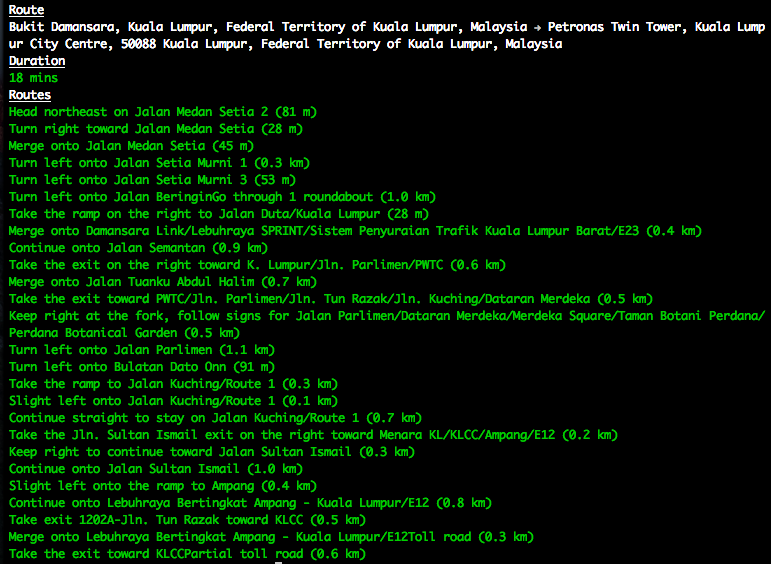
\includegraphics[width=0.825\linewidth]{googlemapscli}
    \caption[Contoh penggunaan perkakas \googlemapscli]{Contoh penggunaan perkakas \googlemapscli\protect\footnotemark.}
    \label{fig:similarapps-googlemapscli}
\end{figure}
\footnotetext{Gambar diambil dari \href{https://github.com/yujinlim/google-maps-direction-cli}{https://github.com/yujinlim/google-maps-direction-cli}}

\subsubsection{Permasalahan}
\label{sec:similarapps-googlemapscli-problem}

Seperti tertulis di awal bab ini, perkakas ini juga tidak bisa digunakan. Alasan perkakas ini tidak dapat digunakan lagi-lagi merupakan masalah teknis, yaitu diperbaruinya API Google \textit{Maps}. Lebih spesifiknya, semenjak 2018, Google tidak lagi memperbolehkan penggunaan API Google \textit{Maps} tanpa kunci API, yang sayangnya mendasari pemakaian perkakas ini. Selain itu, ada ketentuan tambahan dari Google bahwa bahwa kunci API ini tidak lagi bisa didapatkan tanpa membayarkan sebuah biaya tertentu. Oleh karena itu, perkakas ini dianggap tidak bisa dijalankan.

\section{Analisis API KIRI}
\label{sec:analysis-kiri}

API KIRI memiliki tiga buah layanan, yaitu \textit{search place}, \textit{routing}, dan \textit{smart direction}. Di antara ketiga layanan ini, perlu diingat bahwa \textit{smart direction} merupakan sebuah layanan yang bekerja dengan langsung membuka halaman \textit{web} KIRI sendiri, sehingga layanan ini tidak akan digunakan dalam pembuatan perkakas \cl untuk skripsi ini.

\subsection{\textit{Search Place}}
\label{sec:analysis-kiri-searchplace}

Layanan pertama dari dua layanan yang tersisa merupakan layanan \textit{search place.} Layanan ini merupakan layanan API KIRI yang berfungsi untuk mencari sebuah lokasi, beserta nilai \textit{latitude} dan \textit{longitude}-nya, berdasarkan kata kunci yang diberikan oleh pengguna. Untuk memanfaatkan layanan ini, sebuah permintaan GET harus dikirimkan ke alamat API KIRI. Adapun permintaan tersebut akan memiliki parameter-parameter sebagai berikut.

\begin{itemize}
	\item \verb|version|\\
	Parameter ini merupakan tanda bagi API untuk menggunakan protokol versi 2. Karena kemungkinan nilai untuk parameter ini hanya satu, maka parameter ini pasti bernilai \verb|2|.
	\item \verb|mode|\\
	Parameter ini merupakan mode dari servis/jasa API yang akan digunakan oleh pengguna. Untuk pengunaan layanan \textit{search place}, parameter ini diisi dengan \verb|searchplace|.
	\item \verb|region|\\
	Parameter ini mengatur daerah mana tempat lokasi yang ingin dicari berada. Isi dari parameter ini akan diberikan oleh pengguna pada saat pemakaian perkakas.
	\item \verb|querystring|\\
	Parameter ini akan berisi masukan kata kunci untuk mencari lokasi yang ingin ditemukan.
	\item \verb|apikey|\\
	Parameter ini akan berisi sebuah nilai kunci API yang sudah dibuat sebelumnya, seperti dijelaskan di subbab \ref{sec:kiri-api}, parameter ini akan bernilai \verb|68C...97C|\footnote{Bagian tengah dari kunci API diganti dengan ``...'' untuk alasan keamanan.}.
\end{itemize}

\subsection{\textit{Routing}}
\label{sec:analysis-kiri-findroute}

Layanan kedua dari API ini merupakan fungsi utama dari KIRI sendiri, yaitu pencarian rute dengan menggunakan angkot. Layanan ini akan menerima dua buah lokasi yang ingin dijadikan lokasi awal dan lokasi akhir, dan menunjukkan langkah-langkah yang harus ditempuh untuk menempuh perjalanan tersebut, dengan memanfaatkan jasa angkot yang ada. Sama seperti layanan \textit{search place}, layanan ini juga digunakan dengan mengirimkan permintaan GET ke alamat API KIRI.

\begin{itemize}
	\item \verb|version|\\
	Sama seperti pada layanan \textit{search place}, parameter ini hanya dapat diisi dengan nilai \verb|2|.
	\item \verb|mode|\\
	Parameter ini merupakan mode dari servis/jasa API yang akan digunakan oleh pengguna. Untuk penggunaan layanan \textit{routing}, parameter ini diisi dengan \verb|findroute|.
	\item \verb|locale|\\
	Isi dari parameter ini akan ditentukan pada saat pemakaian perkakas.
	\item \verb|start|\\
	Parameter ini merupakan nilai \latlon dari titik awal perjalanan pengguna, yang akan diberikan sebagai masukan pada saat pemakaian perkakas.
	\item \verb|finish|\\
	Parameter ini merupakan nilai \latlon dari titik akhir/tujuan perjalanan pengguna, yang akan diberikan sebagai masukan pada saat pemakaian perkakas.
	\item \verb|presentation|\\
	Parameter ini hanya digunakan untuk fitur \textit{backwards compatibility}. Jika parameter ini ingin digunakan, maka isi dari parameter ini hanya ada satu kemungkinan, yaitu \verb|desktop|. Parameter ini ada karena versi lama dari halaman \textit{web} KIRI memerlukan tampilan yang berbeda untuk perangkat-perangkat \textit{desktop} dan perangkat-perangkat \textit{mobile}. Walaupun begitu, sekarang parameter ini tidak lagi berpengaruh ke keluaran API.
	\item \verb|apikey|\\
	Sama seperti pada layanan \textit{search place}, parameter ini akan berisi sebuah nilai kunci API yang sudah dibuat sebelumnya, yaitu \verb|68C...97C|.
\end{itemize}
\vspace{\baselineskip}\noindent
Layanan ini dapat digunakan sebagai lanjutan dari layanan \textit{search place}, terutama karena fitur pencarian rute hanya menerima nilai \latlon dari lokasi-lokasi yang akan digunakan sebagai masukan, yang tidak hanya akan menyusahkan pengguna dalam memakai perkakas \cl ini, tetapi juga kedua nilai tersebut juga merupakan salah satu dari keluaran layanan pencarian lokasi. Jadi, dengan menggunakan kedua layanan tersebut secara berurutan, maka pengguna akan bisa mencari lokasi awal dan akhir yang diinginkan hanya dengan kata-kata kunci, dan selanjutnya pengguna akan dapat menerima langkah-langkah yang harus ditempuh dalam rute sebagai keluaran akhir dari perkakas.

\section{Analisis Perkakas yang Dibuat}
\label{sec:analysis-thesisapp}

Di bagian ini akan dibahas analisis hal-hal yang berhubungan dengan perkakas yang dibangun sebagai proyek skripsi ini.

\subsection{Analisis Fitur Perkakas}
\label{sec:analysis-thesisapp-features}

Pada skripsi ini, akan dibangun sebuah aplikasi berupa perkakas \cl\xspace yang merupakan ekstensi dari sebuah aplikasi berbasis \textit{web} lain, yaitu KIRI. Perkakas ini akan menjadi ekstensi KIRI dengan cara memungkinkan penggunanya untuk mengakses fungsi-fungsi API KIRI dari \cl\xspace milik perangkat mereka masing-masing. Fungsi utama dari perkakas ini tentunya sama dengan KIRI sendiri, yaitu membantu navigasi dari satu lokasi ke lokasi lain dengan menggunakan angkot.

Walaupun begitu, aplikasi ini akan memiliki tiga fitur utama yang berhubungan satu sama lain, yaitu pencarian lokasi dengan kata kunci pencarian, pencarian rute dengan koordinat \latlon\xspace lokasi awal dan akhir, dan pencarian rute dengan kata kunci pencarian lokasi awal dan akhir. Selain ketiga fitur utama ini, perkakas juga akan memiliki fitur untuk menampilkan halaman bantuan penggunaannya, seperti layaknya perkakas \cl\xspace pada umumnya.

\begin{itemize}
	\item Pencarian lokasi dengan kata kunci pencarian\\
	Pencarian lokasi merupakan fungsi pertama dari perkakas ini. Untuk fungsi ini, masukan langsung dari pengguna yang akan diterima oleh perkakas adalah kata kunci dari sebuah lokasi yang ingin dicari. Kemudian, perkakas akan memprosesnya melalui API KIRI, lalu mengembalikan nama lokasi tersebut, serta nilai \latlon -nya, sebagai keluaran akhir dari proses tersebut.
	\vfill\newpage % prevent widow on second next page
	\item Pencarian rute angkot dengan koordinat \latlon\xspace lokasi awal dan akhir\\
	Pencarian rute angkot dengan koordinat merupakan fungsi kedua dari perkakas ini. Dalam fungsi ini, perkakas akan meminta masukan dari pengguna berupa nilai \latlon\xspace dari lokasi awal serta lokasi akhir dari perjalanan pengguna. Setelah masukan ini berhasil diterima dan diproses, perkakas akan mengeluarkan keluaran akhir berupa langkah-langkah yang harus diambil oleh pengguna untuk pergi dari lokasi awal ke lokasi akhir, dengan memanfaatkan jasa angkot yang ada.
	\item Pencarian rute angkot dengan kata kunci pencarian lokasi awal dan akhir\\
	Pencarian rute angkot dengan kata kunci pencarian merupakan fungsi ketiga  dari perkakas ini. Dalam fungsi ini, perkakas akan meminta masukan dari pengguna berupa kata kunci untuk pencarian lokasi awal dan lokasi akhir dari perjalanan yang ingin dilakukan. Setelah masukan ini berhasil diterima dan diproses, perkakas akan langsung mengeluarkan keluaran akhir berupa langkah-langkah yang harus diambil oleh pengguna untuk pergi dari lokasi awal ke lokasi akhir, dengan memanfaatkan jasa angkot yang ada.
\end{itemize}
\vspace{\baselineskip}\noindent % Prevent widow on next page
Selain itu, perkakas ini juga akan memiliki fitur-fitur standar yang harus dimiliki oleh perkakas-perkakas \cl, seperti dokumentasi singkat (bantuan penggunaan perkakas) sebagai salah satu mode operasional perkakas, dan juga \textit{man page} (khusus implementasi di Linux).

\subsubsection{Aturan Penamaan}
\label{sec:analysis-thesisapp-features-conventions}

Untuk memenuhi fitur-fitur tersebut, perkakas akan perlu berbagai opsi yang masing-masing merepresentasikan fitur (mode operasional) perkakas, serta variabel-variabel yang dibutuhkan oleh API. Setelah dilakukan analisis perkakas-perkakas sejenis yang memerlukan opsi-opsi dalam masukannya, dibuat seperangkat aturan yang mendasari penamaan dari opsi-opsi yang akan dimiliki perkakas yang akan dibuat. Berikut merupakan aturan-aturan tersebut.

\begin{enumerate}
	\item Opsi-opsi perkakas yang akan dibuat akan dinamakan berdasarkan penamaan opsi-opsi dalam perkakas-perkakas yang telah dianalisis. Hal ini juga berarti bahwa nama-nama opsi perkakas yang akan dibuat kemungkinan besar tidak akan sama dengan nama opsi-opsi perkakas-perkakas yang dianalisis.
	\item Nama pendek (satu huruf) opsi umumnya akan dinamakan sesuai dengan huruf pertama dari fitur/variabel yang direpresentasikan oleh opsi tersebut.
	\item Nama panjang dari opsi umumnya akan dinamakan sesuai dengan nama fitur/variabel yang direpresentasikan oleh opsi tersebut.
	\item Argumen dari opsi yang merepresentasikan fitur perkakas akan dinamakan sesuai dengan nama dari mode operasionalnya masing-masing di API KIRI, kecuali \texttt{direct}, karena fitur ini merupakan mode tambahan yang bukan merupakan fitur langsung dari API KIRI.
	\item Nama-nama opsi dan, baik pendek maupun panjang, yang jika mengikuti ketiga aturan pertama akan menghasilkan nama yang sama dengan nama opsi lain, akan dinamakan dengan nama buatan yang artinya tidak terlalu jauh dengan variabel apa yang direpresentasikan olehnya.
\end{enumerate}

\subsubsection{Opsi-opsi Perkakas}
\label{sec:analysis-thesisapp-features-options}

Mengikuti aturan-aturan yang sudah dipaparkan di sub-subbab sebelumnya, berikut merupakan daftar serta penjelasan singkat dari opsi-opsi yang akan disediakan dalam perkakas yang akan dibangun.

\begin{itemize}
	\item \verb|-h (--help)|\\
	Perlu diingat juga bahwa aplikasi ini merupakan aplikasi \cl\xspace murni, yang berarti bahwa seluruh operasi dari aplikasi ini akan dilakukan tanpa bantuan gambar grafis apa pun, sehingga perintah untuk menunjukkan apa perintah-perintah dan opsi-opsi yang tersedia merupakan sebuah keharusan. Hal ini merupakan fungsi satu-satunya dari perintah ini. Mengikuti nama opsi-opsi bantuan dari perkakas-perkakas yang telah dianalisis, maka opsi ini akan dinamakan \verb|--help|, atau \verb|-h| untuk versi pendeknya.
	
	\item \verb|-m <mode> (--mode)|\\
	Opsi ini merupakan opsi berparameter yang menentukan fitur mana yang ingin digunakan oleh pengguna. Nama dari opsi ini ditentukan sebagai \verb|-m| atau \verb|--mode| karena opsi ini merupakan opsi yang mengatur mode penggunaan perkakas. Adapun isi dari parameter \verb|<mode>| yang dapat digunakan adalah sebagai berikut:
	
	\begin{itemize}	
		\item \verb|searchplace|\\
		Parameter ini akan menandakan bahwa pengguna ingin menggunakan fitur \textit{search place} dari perkakas. Untuk mode ini, perkakas akan menerima input dari pengguna dalam bentuk parameter-parameter dari opsi-opsi tambahan. Adapun opsi-opsi tersebut adalah sebagai berikut.
			
		\begin{itemize}
			\item \verb|-r <region> (--region)|\\
			Opsi ini merupakan opsi yang akan menerima parameter berupa kode area (region) dari lokasi yang ingin dicari.
			\item \verb|-q <kata kunci> (--query)|\\
			Opsi ini merupakan opsi yang akan menerima sebuah \textit{string} sebagai parameternya. \textit{String} ini akan digunakan oleh perkakas sebagai kata kunci untuk pencarian lokasi yang ingin ditemukan oleh pengguna. Opsi ini diberi nama demikian karena nama parameter ini di API KIRI adalah ``\verb|querystring|''.
			\item \verb|-l <kode bahasa> (--locale)|\\
			Opsi ini akan menerima parameter yang mengatur bahasa (\textit{locale}) yang akan digunakan oleh perkakas di keluarannya nanti. Opsi ini merupakan tambahan spesifik dari perkakas ini, karena keluaran dari perkakas mengandung kata-kata yang bukan merupakan nama/koordinat lokasi hasil. Walaupun begitu, opsi ini tidak akan mempengaruhi nama lokasi dalam keluaran.
		\end{itemize}

		\item \verb|findroute|\\
		Parameter ini akan menandakan bahwa pengguna ingin menggunakan fitur \textit{find route} dari perkakas. Sama seperti mode \verb|searchplace|, perkakas akan menerima input dari pengguna dari parameter-parameter milik opsi-opsi tambahan. Adapun opsi-opsi tersebut adalah sebagai berikut.
		
		\begin{itemize}
			\item \verb|-s <lokasi awal> (--start)|\\
			Opsi ini merupakan opsi yang akan menerima parameter berupa lokasi awal (\textit{start}) perjalanan pengguna nantinya. Opsi ini hanya menerima masukan lokasi berupa nilai \latlon\xspace dari lokasi tersebut.
			\item \verb|-f <lokasi akhir> (--finish)|\\
			Opsi ini merupakan opsi yang akan menerima parameter berupa lokasi akhir (\textit{finish}) perjalanan pengguna nantinya. Sama seperti opsi sebelumnya, parameter ini juga hanya menerima masukan lokasi berupa nilai \latlon.
			\item \verb|-l <kode bahasa> (--locale)|\\
			Opsi ini akan menerima parameter yang mengatur bahasa yang akan digunakan oleh perkakas di keluarannya nanti. Opsi ini adalah opsi yang sama dengan opsi yang digunakan dalam mode \verb|searchplace|, dan mengikuti aturan penamaan yang sama.
		\end{itemize}
		
		\item \verb|direct|\\
		Parameter ini merupakan tambahan fitur spesifik untuk perkakas ini, yang merupakan gabungan dari fitur pencarian lokasi dan pencarian rute. Fitur ini akan menggabungkan kedua fitur tersebut dengan langkah-langkah berikut.
		
		\begin{enumerate}
			\item Perkakas akan menerima lokasi awal dan akhir berupa kata kunci dari pengguna yang dimasukkan ke dalam parameter dari opsi masing-masing.
			\item Pencarian lokasi akan dilakukan dua kali\textemdash untuk lokasi awal dan lokasi akhir, dan hasilnya akan langsung ditampilkan ke pengguna. Perlu ditekankan bahwa:
			\newpage\vspace*{-1.5em} % prevent hanging widow
			\begin{itemize}
				\item Perkakas hanya akan mengambil hasil pertama saja di tiap pencariannya, jadi jika terdapat banyak hasil dari salah satu proses pencarian, hanya lokasi pertama saja yang akan digunakan untuk proses selanjutnya.
				\item Perkakas tidak peduli apakah hasil pencarian tersebut benar merupakan hasil yang diinginkan pengguna atau tidak. Jika satu atau lebih lokasi ternyata tidak sesuai, pengguna dapat melakukan ulang seluruh prosesnya.
			\end{itemize}
			
			\item Koordinat \latlon\xspace dari kedua lokasi tersebut kemudian akan digunakan sebagai masukan untuk langkah kedua dari fitur ini, yaitu pencarian rute.
			\item Hasil dari pencarian rute akan ditampilkan sebagai keluaran akhir dari fitur ini.
		\end{enumerate}
		\noindent
		Secara esensi, fitur ini merupakan fitur yang didesain untuk bekerja menyerupai fitur \textit{smart direction}, yang merupakan salah satu fitur dari KIRI sendiri, tetapi bukan merupakan fitur yang dapat digunakan melalui API KIRI. Adapun parameter yang diperlukan untuk fitur ini merupakan gabungan dari opsi-opsi kedua fitur sebelumnya, yaitu:
		
		\begin{itemize}
			\item \verb|-S <region tempat lokasi awal berada> (--regstart)|\\
			Opsi ini akan menerima parameter berupa kode region dari lokasi awal. Opsi ini tidak dapat diberi huruf \verb|-r| seperti pada mode \verb|searchplace|, karena pemberian nama tersebut akan membuat konflik dengan opsi kode region lokasi akhir. Oleh karena itu, opsi ini diberikan huruf \verb|-S| (s kapital), dengan nama panjang \verb|--regstart|, yang berarti ``\textit{region start}''.
			\item \verb|-F <region tempat lokasi akhir berada> (--regfinish)|\\
			Opsi ini akan menerima parameter berupa kode region dari lokasi akhir. Opsi ini tidak dapat diberi huruf \verb|-r| seperti pada mode \verb|searchplace|, karena pemberian nama tersebut akan membuat konflik dengan opsi kode region lokasi awal. Oleh karena itu, opsi ini diberikan huruf \verb|-F| (f kapital), dengan nama panjang \verb|--regfinish|, yang berarti ``\textit{region finish}''.
			\item \verb|-s <kata kunci untuk lokasi awal> (--start)|\\
			Opsi ini akan menerima parameter berupa kata kunci untuk pencarian lokasi awal yang akan digunakan. Penamaan opsi ini sama seperti opsi ekuivalennya di mode \verb|findroute|.
			\item \verb|-f <kata kunci untuk lokasi akhir> (--finish)|\\
			Opsi ini akan menerima parameter berupa kata kunci untuk pencarian lokasi akhir yang akan digunakan. Penamaan opsi ini sama seperti opsi ekuivalennya di mode \verb|findroute|.
			\item \verb|-l <kode bahasa> (--locale)|\\
			Opsi ini akan menerima parameter yang mengatur bahasa yang akan digunakan oleh perkakas di keluarannya nanti. Opsi ini merupakan opsi yang sama dengan opsi yang digunakan dalam kedua mode lainnya, dan juga mengikuti aturan penamaan yang sama.
		\end{itemize}
		
	\end{itemize}
	
\end{itemize}
\vspace{-0.5em} % prevent hanging widow
\subsection{Analisis Kebutuhan Perkakas}
\label{sec:analysis-thesisapp-usecases}

Perkakas \cl\xspace ini akan memiliki tiga fitur utama, yaitu pencarian lokasi dengan kata kunci, pencarian rute dengan koordinat \latlon\xspace lokasi, dan pencarian rute dengan kata kunci pencarian lokasi. Oleh karena itu, diagram \textit{use case} dari aplikasi ini akan mengandung empat \textit{use case}, yang dapat dilihat di Gambar \ref{fig:thesisapp-uml}. 

Berikut merupakan empat tabel \textit{scenario case}, yang masing-masing akan menjelaskan secara singkat keempat \textit{use case} dari perkakas yang dibuat. Tabel-tabel tersebut adalah sebagai berikut.

\begin{itemize}
	\item Tabel \ref{tab:thesisapp-scenariocase-help}: \textit{Scenario case} untuk fitur penampilan bantuan penggunaan perkakas.
	\item Tabel \ref{tab:thesisapp-scenariocase-searchplace}: \textit{Scenario case} untuk fitur pencarian lokasi dengan kata kunci pencarian.
	\item Tabel \ref{tab:thesisapp-scenariocase-findroute}: \textit{Scenario case} untuk fitur pencarian rute dengan \latlon\xspace lokasi awal dan akhir.
	\item Tabel \ref{tab:thesisapp-scenariocase-directroute}: \textit{Scenario case} untuk fitur pencarian rute dengan kata kunci pencarian lokasi awal dan akhir.
\end{itemize}

\begin{figure}[H]
    \centering
    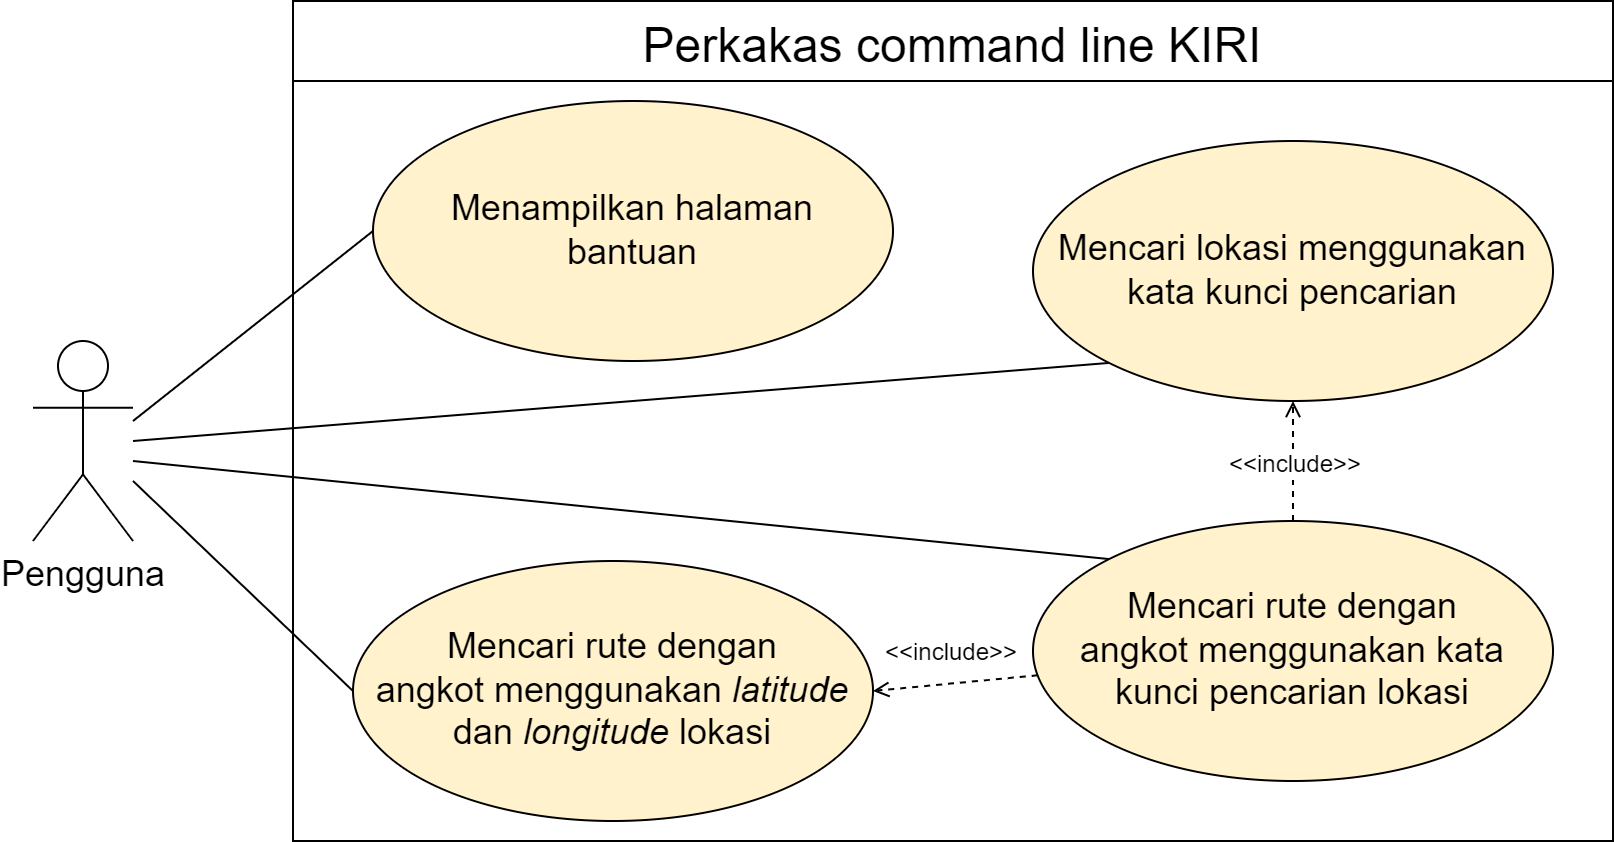
\includegraphics[width=0.875\linewidth]{thesisapp-uml}
    \caption[Diagram \textit{use case} perkakas yang dibangun]{Diagram \textit{use case} dari perkakas yang dibangun.}
    \label{fig:thesisapp-uml}
\end{figure}

\begin{longtable}{| l | c p{10cm} |}
	\caption{\textit{Scenario case} untuk fitur halaman bantuan.} 
	\label{tab:thesisapp-scenariocase-help} \\
	
	\hline 
	\endfirsthead
	
	\multicolumn{3}{c}{\textbf{\tablename\ \thetable{}} --- Lanjutan dari halaman sebelumnya} \\
	\hline 
	\endhead
	
	\hline \multicolumn{3}{|r|}{{Lanjut di halaman berikutnya...}} \\ \hline
	\endfoot
	
	\hline
	\endlastfoot

        \textbf{Nama} & \multicolumn{2}{p{10.5cm} |}{Menampilkan halaman bantuan} \\
    \hline \addlinespace[0.1cm]
    \hline
        \textbf{Deskripsi} & \multicolumn{2}{p{10.5cm} |}{Fitur untuk menampilkan bantuan penggunaan perkakas.} \\
    \hline
		\textbf{Aktor} & \multicolumn{2}{p{10.5cm} |}{Pengguna aplikasi} \\
	\hline
		\textbf{Pre-kondisi} & \multicolumn{2}{p{10.5cm} |}{-} \\
    \hline
		\textbf{Pos-kondisi} & \multicolumn{2}{p{10.5cm} |}{Halaman bantuan penggunaan.} \\
    \hline
		\textbf{Skenario utama} & 1. & Perkakas membaca masukan pengguna, yaitu perintah untuk menampilkan bantuan penggunaan perkakas. \\
		 & 2. & Perkakas menampilkan bantuan penggunaan perkakas kepada pengguna. \\
    \hline
		\textbf{Skenario eksepsi} & \multicolumn{2}{p{10.5cm} |}{Perintah yang dimasukkan pengguna tidak sesuai format/tidak valid.} \\
\end{longtable}

\begin{longtable}{| l | c p{10cm} |}
	\caption{\textit{Scenario case} untuk fitur pencarian lokasi dengan kata kunci pencarian.} 
	\label{tab:thesisapp-scenariocase-searchplace} \\
	
	\hline 
	\endfirsthead
	
	\multicolumn{3}{c}{\textbf{\tablename\ \thetable{}} --- Lanjutan dari halaman sebelumnya} \\
	\hline 
	\endhead
	
	\hline \multicolumn{3}{|r|}{{Lanjut di halaman berikutnya...}} \\ \hline
	\endfoot
	
	\hline
	\endlastfoot

        \textbf{Nama} & \multicolumn{2}{p{10.5cm} |}{Mencari lokasi menggunakan kata kunci pencarian} \\
    \hline \addlinespace[0.1cm]
    \hline
        \textbf{Deskripsi} & \multicolumn{2}{p{10.5cm} |}{Fitur untuk mencari lokasi di area tertentu berdasarkan kata kunci pencarian.} \\
    \hline
		\textbf{Aktor} & \multicolumn{2}{p{10.5cm} |}{Pengguna aplikasi} \\
	\hline
		\textbf{Pre-kondisi} & \multicolumn{2}{p{10.5cm} |}{-} \\
    \hline
		\textbf{Pos-kondisi} & \multicolumn{2}{p{10.5cm} |}{Nama dari lokasi serta koordinat \textit{latitude} dan \textit{longitude}-nya ditampilkan kepada pengguna.} \\
    \hline
		\textbf{Skenario utama} & 1. & Perkakas membaca masukan berupa kata kunci pencarian lokasi dari argumen dalam perintah \cl. \\
		 & 2. & Perkakas memproses masukan tersebut dan mengirimkannya ke API KIRI untuk diproses lebih lanjut. \\
		 & 3. & Perkakas menerima keluaran berupa nama serta koordinat \latlon\xspace dari lokasi yang ditemukan. \\
		 & 4. & Perkakas menampilkan kembali keluaran tersebut kepada pengguna. \\
    \hline
		\textbf{Skenario eksepsi} & - &  Pengguna memasukkan masukan yang tidak valid sebagai kata kunci pencarian. \\
		 & - & Lokasi tidak berhasil ditemukan. \\
\end{longtable}

\begin{longtable}{| l | c p{10cm }|}
	\caption{\textit{Scenario case} untuk fitur pencarian rute dengan angkot, dengan nilai \latlon\xspace kedua lokasi sebagai masukan.}
    \label{tab:thesisapp-scenariocase-findroute} \\
	
	\hline 
	\endfirsthead
	
	\multicolumn{3}{c}{\textbf{\tablename\ \thetable{}} --- Lanjutan dari halaman sebelumnya} \\
	\hline 
	\endhead
	
	\hline \multicolumn{3}{|r|}{{Lanjut di halaman berikutnya...}} \\ \hline
	\endfoot
	
	\hline
	\endlastfoot

        \textbf{Nama} & \multicolumn{2}{p{10.5cm} |}{Mencari rute dengan angkot menggunakan \latlon\xspace lokasi} \\
    \hline \addlinespace[0.1cm]
    \hline
        \textbf{Deskripsi} & \multicolumn{2}{p{10.5cm} |}{Fitur untuk mencari cara pergi ke satu lokasi ke lokasi lainnya dengan menggunakan angkot dengan nilai \latlon\xspace lokasi sebagai masukan.} \\
    \hline
		\textbf{Aktor} & \multicolumn{2}{p{10.5cm} |}{Pengguna aplikasi} \\
	\hline
		\textbf{Pre-kondisi} & \multicolumn{2}{p{10.5cm} |}{-} \\
    \hline
		\textbf{Pos-kondisi} & \multicolumn{2}{p{10.5cm} |}{Langkah-langkah yang harus ditempuh untuk perjalanan \mbox{tersebut} akan ditampilkan kepada pengguna.} \\
    \hline
		\textbf{Skenario utama} & 1. & Perkakas membaca masukan berupa nilai \textit{latitude} dan \mbox{\textit{longitude}} lokasi awal dan akhir dari argumen dalam \mbox{perintah} \cl. \\
		 & 2. & Perkakas memproses masukan tersebut dan mengirimkannya ke API KIRI untuk diproses lebih lanjut. \\
		 & 3. & Perkakas menerima keluaran akhir dari API KIRI berupa langkah-langkah dalam rute yang perlu ditempuh. \\
		 & 4. & Perkakas menampilkan kembali keluaran tersebut kepada pengguna. \\
	\hline
		\textbf{Skenario eksepsi} & - & Pengguna memasukkan masukan yang tidak valid sebagai kata kunci pencarian. \\
		 & - & Rute tidak berhasil ditemukan/tidak tersedia. \\
\end{longtable}

\begin{longtable}{| l | c p{10cm} |}
	\caption{\textit{Scenario case} untuk fitur pencarian rute dengan angkot, dengan kata kunci pencarian lokasi awal dan akhir sebagai masukan.}
    \label{tab:thesisapp-scenariocase-directroute} \\
	
	\hline 
	\endfirsthead
	
	\multicolumn{3}{c}{\textbf{\tablename\ \thetable{}} --- Lanjutan dari halaman sebelumnya} \\
	\hline 
	\endhead
	
	\hline \multicolumn{3}{|r|}{{Lanjut di halaman berikutnya...}} \\ \hline
	\endfoot
	
	\hline
	\endlastfoot

        \textbf{Nama} & \multicolumn{2}{p{10.5cm} |}{Mencari rute dengan angkot menggunakan kata kunci pencarian lokasi} \\
    \hline \addlinespace[0.1cm]
    \hline
        \textbf{Deskripsi} & \multicolumn{2}{p{10.5cm} |}{Fitur untuk mencari cara pergi ke satu lokasi ke lokasi \mbox{lainnya} dengan menggunakan angkot dengan dengan kata kunci \mbox{pencarian} kedua lokasi sebagai masukan.} \\
    \hline
		\textbf{Aktor} & \multicolumn{2}{p{10.5cm} |}{Pengguna aplikasi} \\
	\hline
		\textbf{Pre-kondisi} & \multicolumn{2}{p{10.5cm} |}{-} \\
    \hline
		\textbf{Pos-kondisi} & \multicolumn{2}{p{10.5cm} |}{Langkah-langkah yang harus ditempuh untuk perjalanan \mbox{tersebut} akan ditampilkan kepada pengguna.} \\
    \hline
		\textbf{Skenario utama} & 1. & Perkakas membaca masukan berupa kata kunci pencarian lokasi awal dan akhir dari argumen dalam perintah \cl. \\
		 & 2. & Perkakas memproses kata kunci pencarian lokasi awal dan mengirimkannya ke API KIRI untuk diproses lebih lanjut. \\
		 & 3. & Perkakas menerima keluaran berupa koordinat \latlon\xspace lokasi awal dari API KIRI. \\
		 & 4. & Perkakas memproses kata kunci pencarian lokasi akhir dan mengirimkannya ke API KIRI untuk diproses lebih lanjut. \\
		 & 5. & Perkakas menerima keluaran berupa koordinat \latlon\xspace lokasi akhir dari API KIRI. \\
		 & 6. & Perkakas mengirimkan kedua nilai \latlon\xspace lokasi ke API KIRI sebagai masukan dari proses pencarian rute. \\
		 & 7. & Perkakas menerima keluaran akhir dari API KIRI berupa langkah-langkah dalam rute yang perlu ditempuh. \\
		 & 8. & Perkakas menampilkan kembali keluaran tersebut kepada pengguna. \\
	\hline
		\textbf{Skenario eksepsi} & - & Pengguna memasukkan masukan yang tidak valid di dalam salah satu parameter. \\
		 & - & Lokasi yang dicari dalam langkah 2 atau langkah 4 tidak ditemukan. \\
		 & - & Rute tidak berhasil ditemukan/tidak tersedia. \\
\end{longtable}
